\documentclass[11pt,a4paper]{article}
\usepackage[margin=24mm]{geometry}
\usepackage{fontspec,unicode-math,booktabs,graphicx,hyperref}
\setmainfont{STIXGeneral}\setmathfont{STIX Two Math}\hypersetup{hidelinks}
\title{A complete comparison for five Topic B manuscripts}
\author{Human Compression Project}\date{11 October 2026}
\begin{document}\maketitle
Topic B now compares N001, N003, N008, L030 and L040. The new original is Fernandes--Leemans, \emph{C-groups of high rank for the symmetric groups}: the accepted institutional manuscript contains twenty authored pages and one publisher cover. The comparison uses that exact edition, not the earlier arXiv PDF. Five originals are counted; the thirty-five new detailed clauses are not thirty-five papers.

\paragraph{The full topic.}
Every earlier source and complete application remains. The existing five-page common paper is retained in full, as is the new ten-page common paper. The new application has eleven pages and its four whole programs fill a seven-page appendix. No overlap between the common papers is deducted before a revised unified proof is reviewed.
\begin{center}\begin{tabular}{lr}\toprule
Complete component & NFC nonspace characters\\\midrule
All five originals & 124,906\\
Earlier common paper & 14,124\\
New common paper & 28,423\\
All five applications & 76,243\\
Full printed program appendix & 13,170\\
Full raw programs, alternative representation & 12,330\\\bottomrule
\end{tabular}\end{center}
Writing $U$ for \emph{both entire common papers}, $A_i$ for each complete application and $P$ for the full program bundle gives
\[
R_{\rm written}=\frac{\sum_i c(L_i)}{c(U)+\sum_i c(A_i)}=1.051.
\]
Including all printed programs gives 0.947; using all raw programs instead gives 0.953. Printed and raw code are alternatives, never a duplicate charge. The primary written replacement is slightly shorter overall, but the complete replacement including either program representation is longer.

\paragraph{Applications after acquisition.}
Each conditional factor below is $r_i\mid(U,P)=c(L_i)/c(A_i)$. It assumes that \emph{both entire common papers and all four complete programs have already been acquired}. It is not a whole-topic saving.
\begin{center}\begin{tabular}{lllrr}\toprule
Original & Application & Original cost & Application cost & Conditional\\\midrule
N001 & B1 & 14,519 & 7,371 & 1.970 \\
N003 & B2 & 17,780 & 14,170 & 1.255 \\
N008 & B3 & 18,009 & 11,132 & 1.618 \\
L030 & B4 & 22,704 & 12,286 & 1.848 \\
L040 & B5 & 51,894 & 31,284 & 1.659 \\
\bottomrule\end{tabular}\end{center}
One program supplies required finite primitive-group inputs, two validate written uniform calculations, and one supports the auxiliary degree-eight example and validates branching. All four are included in the code columns above. Two operational drivers (10,902 and 7,708) and the partial Lean source (4,668) are separately inventoried. Eight new declarations do not formalize the complete classification.
\newpage
\begin{center}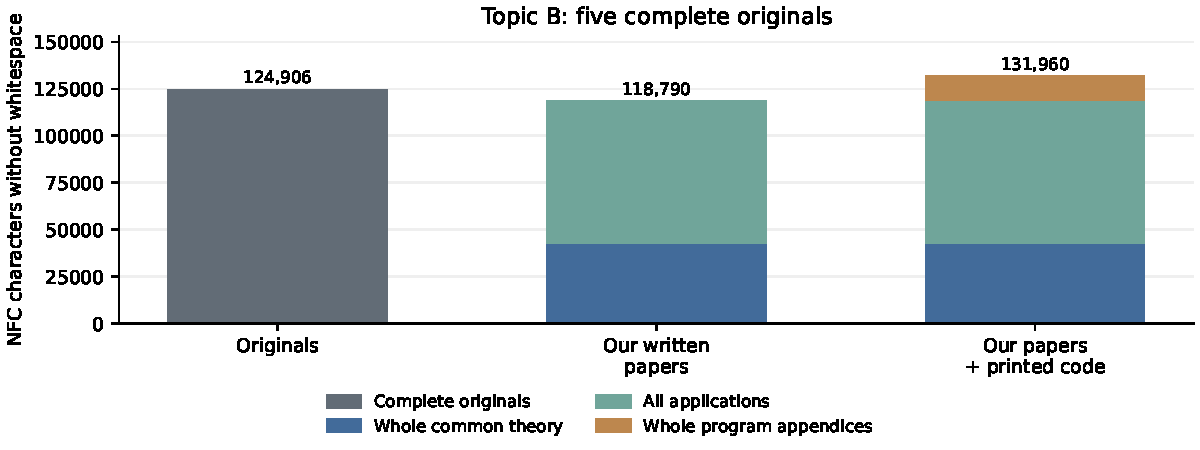
\includegraphics[width=\textwidth]{whole_costs.pdf}\end{center}
The primary representation is unchanged: complete literal authored text for N001 and raw untrimmed PDF extraction for every other original and replacement. Page furniture and the L040 cover remain. Full graphics, historical software, retained outside proofs, primitive-catalogue construction and complete formalization have unknown costs, not zero.

\begin{center}\small\begin{tabular}{lrrr}\toprule
NFC unit & Written & With printed code & With raw code\\\midrule
Whitespace tokens & 1.086 & 1.041 & 1.047 \\
Alphanumeric runs & 1.191 & 1.087 & 1.093 \\
Nonspace characters & 1.051 & 0.947 & 0.953 \\
Collapsed characters & 1.058 & 0.963 & 0.969 \\
Collapsed UTF-8 bytes & 0.994 & 0.912 & 0.918 \\
\bottomrule\end{tabular}\end{center}
In the NFC UTF-8 coordinate, even the written factor is below one. All five units, NFC and NFKC, and three variants---raw untrimmed, raw selected and calibrated selected---remain in the exact data. Thirty coordinates give 240 main fractions. A separate cover-only sensitivity uses all twenty directly extracted authored L040 pages, never token subtraction, and changes no replacement cost. Its primary whole written factor is 1.045; with printed code it is 0.941 and with raw code 0.947. The L040 conditional becomes 1.634. The other four conditional values are unchanged. This sensitivity has 120 additional fractions.

\paragraph{Scope and representation limits.}
The accepted contract recovers the rank $n-1$ classification for $n\geq7$, rank $n-2$ for $n\geq9$, all allowed branching, complete intersection and flag arguments, and corrected general marking presentations. A printed branching clause has a literal counterexample and is not claimed as recovered without correction. The ancillary exact primitive-rank census and the ambiguous leaf-count convention remain outside the stated contract. The source's Whiston, Cameron--Cara and Mar\'oti inputs retain their exact hypotheses and attributions; unavailable full texts and outside computations are not silently free measured proofs.

The distinct input review inspected all forty-nine pages in the input packet and the actual exceptional glyphs. Twenty-four curved diagram classes remain literal extracted names rather than guessed arc symbols. Straight strokes and script letters use only observed outline corrections in the calibrated sensitivity; full graph structure and watermark artwork are not encoded by these text counts. The raw primary is unchanged. No new scientific or conjecture credit follows from this numerical update, and no sawtooth or minimum proof complexity conclusion is inferred from a length ratio. Earlier numerical reports remain immutable. Distinct review of arithmetic and the actual plots is required before admission.
\end{document}
